\documentclass[11pt]{article}
\usepackage{classTools}

\draftfalse

\begin{document}

\psHeader{6}{Wed Oct. 26, 2022 (11:59pm)}

\textbf{Your name: }

\textbf{Collaborators: }

\textbf{No. of late days used on previous psets: }

\textbf{No. of late days used after including this pset: }

\begin{enumerate}
 \item (Matching Algorithms) 

 One practical application of matching algorithms is planning logistics, like in the following example from (fictional) ridesharing service Lyber in (real) New York City's Times Square.  When a customer books a Lyber ride, the ride request is sent to a Lyber server and combined with others to create a schematic 

 like the one drawn in the map below:


\begin{figure}[H]
    \centering
    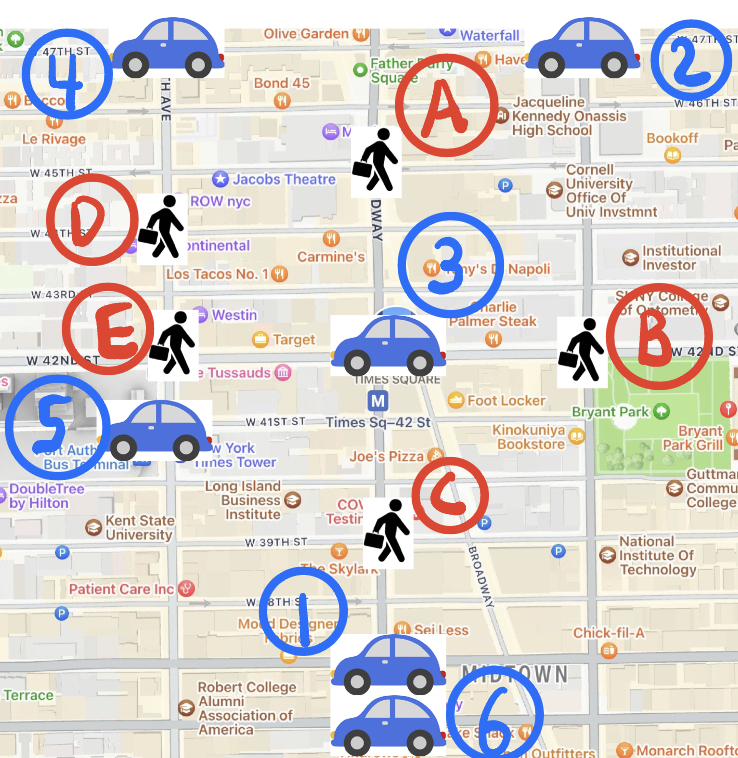
\includegraphics[width=0.87\textwidth]{NYC-map-zoomed-light.jpeg}
    \label{fig:travel_time_graph}
\end{figure}

Given a schematic like this, Lyber's goal is to serve as many customers (labeled A--E in the map) as possible, by assigning each one to a driver (labeled 1--6 in the map). For simplicity, each customer and driver is at an intersection, and assume driving between adjacent streets (vertical segment) takes 30 seconds, and driving between adjacent avenues (horizontal segments) takes 1 minute. However, the one twist is that they want to make sure that \textit{no customer is waiting for longer than 2 minutes}.  They also do not want to assign a driver to more than one customer at once, since serving a single customer can take more than 2 minutes.

    \begin{enumerate}
    \item To perform the assignment, they reduce to Maximum Matching in bipartite graphs.  Draw a bipartite graph corresponding to the drivers and customers in the map above.

    
    \item The Lyber app first prioritizes customers on Broadway, so they initially assign customer $A$ to driver 3 and customer $C$ to driver 5. Using the algorithm from class, find a \textit{maximum matching} in the bipartite matching graph you've drawn, starting from the initial matching of $A$ to 3 and $C$ to 5. Draw pictures showing the sequence of matchings and augmenting paths you find. (No need to break down the steps of the algorithm to find the augmenting paths.)


    \item The Lyber app also allows users to schedule trips in advance. One Lyber driver receives the following pre-programmed trips scheduled by 4 different users (all of them need multiple rides on the same day):
    \begin{itemize}
        \item User A: one trip from 10 to 10:29, another from 11 to 11:59, another from 1:15 to 12:29, and another from 13 to 13:29.
        \item User B: one trip from 10:15 to 11:14, another from 11:30 to 12:14, and another from 12:45 to 13:14.
        \item User C: one trip from 10:30 to 11:44, another from 12:30 to 12:59, and another from 13:15 to 13:44.
        \item User D: one trip from 10 to 10:44, another from 11:15 to 11:29, another from 12 to 12:44, and another from 13:30 to 13:59.
    \end{itemize}
    The Lyber driver wants to maximize the total number of different rides, because they earn a fixed rate per ride. (The driver is \textit{not} trying to maximize the driving time). 

    We also assume for simplicity that the driver needs no time to move between different rides (i.e., it is possible that one ride finishes at 10:29 and the next one starts immediately at 10:30). 

    Use a greedy algorithm that we saw in class to find a maximum-sized set of non-conflicting rides.  State which algorithm you are using, how you are applying it to this ride-selection problem, and write down the order in which the greedy algorithm selects the rides in the solution. 

    
    \end{enumerate}

 \item (EthiCS Reflection) 
 Suppose there are two patients in need of an immediate kidney transplant, but only one donor is currently available. The donor’s kidney is compatible with both patients. Patient A is 30 years old, and is expected to live 6 additional years as a result of the transplant. Patient B is 60 years old, and is expected to live 10 additional years as a result of the transplant. {\em All else being equal} (e.g., both patients have an urgent need for the transplant; both patients have been on the kidney exchange waiting list for the same length of time), \underline{\textbf{which patient should the kidney go to, and why?}} Your response should take the form of a short paragraph (3-4 sentence) reflection. {\em In explaining your ethical reasoning about the case, be sure to draw on at least one concept discussed in class.}

 \item (Vertex-Weighted Matching)
        For a graph $G=(V,E)$ and a subset $F\subseteq E$, 

        let $V(F)$ denote the set $\bigcup_{f \in F}f$ of 
        vertices that are an endpoint of at least one edge in $F$.
        \begin{enumerate}
        \item Prove that if $G=(V,E)$ is a graph and $M\subseteq E$ is a matching in $G$, then there is a maximum-size matching $M'$ such that $V(M)\subseteq V(M')$.  (Hint: consider constructing a maximum matching via augmenting paths, but starting with $M_0=M$ rather than $M_0=\emptyset$. What can you say about the $V(M_i)$'s?) \label{part:monotonicity}

        \item   In the Embedded EthiCS module, we saw how simply maximizing the {\em size} of a matching may not always be the right objective.  Thus, it is natural to consider weighted versions of the matching problem. Suppose we
        we consider vertex-weighted graphs $G = (V,E,w)$, $w$ is an array specifying a nonnegative edge weight $w(v)$ for every $v\in V$.  (For example, the weight assigned to a patient might correspond to the number of extra years of life they would gain from a donation.)
          The goal of the {\em vertex-weighted maximum matching problem} is to find a matching $M$ maximizing its {\em total weight} $$w(M) = \sum_{\{u,v\}\in M} (w(u)+w(v)).$$
        (This corresponds to the utilitarian objective discussed in Embedded EthiCS module.)
        Using Part~\ref{part:monotonicity}, prove that every graph $G$ has a matching $M^*$ that simultaneously maximizes both total weight and size.  That is, for every matching $M$ in $G$, we have
        both $w(M)\leq w(M^*)$ and $|M^*|\leq |M|$.

        \item (optional\footnote{This problem won't make a difference between N, L, R-, and R grades. As this problem is purely extra credit, course staff will deprioritize questions about this problem at office hours and on Ed.}) Explain why the same holds for the maximin objective discussed in the Embedded EthiCS module.  That is, there is always a matching $M$ that simultaneously maximizes the maximin objective and $|M|$. 
        \end{enumerate}
        

\item (Edge-Weighted Bipartite Matching) 
  Instead of considering vertex weights, we could instead study matching on
{\em edge-weighted} bipartite graphs $G = (V,E,w)$, where $w$ is an array specifying a nonnegative edge weight $w(e)$ for every $e\in E$.  

   The goal of the {\em edge-weighted maximum matching problem} is to find a matching $M$ maximizing $$w(M) = \sum_{e\in M} w(e).$$
   \begin{enumerate}
    \item Construct an edge-weighted bipartite graph $G = (V,E,w)$ such that there is no matching $M$ in $G$ that simultaneously maximizes the weight $w(M)$ and the size $|M|$.  Thus, there can be an inherent tension between these two objectives. 

    \item (optional\footnotemark[1])
  
    One real-life constraint in kidney exchange is that donors $d$ are often associated with a particular patient $p$ (e.g. a close family member) such that $d$ is only willing to donate a kidney if $p$ receives a kidney from someone.  ($d$ would donate their kidney directly to $p$ if they could, but they are incompatible.) 
    Suppose we have an (unweighted) bipartite graph $G=(V_0\cup V_1,E)$ representing $n$ such donor-patient pairs, i.e. $V_0=\{d_0,d_1,\ldots,d_{n-1}\}$, $V_1 = \{p_0,p_1,\ldots,p_{n-1}\}$, where $p_i$ is the patient associated with donor $d_i$. We assume $\{d_i,p_i\}\notin E$ for each $i$.   Our goal is to find a matching $M$ of the largest possible size $|M|$, subject to the constraint that $d_i$ is matched in $M$ only if $p_i$ is matched in $M$. 

    Show that we can reduce this constrained version of the maximum matching problem to finding a maximum-weight {\em perfect} matching in an appropriate edge-weighted bipartite graph, where
    a perfect matching is a matching that matches all the vertices in the graph. (Hint: add edges $\{d_i,p_i\}$ with appropriate edge weights.) 
    \end{enumerate}

\end{enumerate}
\end{document}